\documentclass[aspectratio=43,english]{beamer} %If you want to create Polish presentation, replace 'english' with 'polish' and uncomment 3-th line, i.e., '\usepackage{polski}'
\usepackage[utf8]{inputenc}
\usepackage{polski} %Uncomment for Polish language
\usepackage{babel}
\usepackage{listings} %We want to put listings

\mode<beamer>{ 	%in 'beamer' mode
	\hypersetup{pdfpagemode=FullScreen}		%Enable Full screen mode
	\usetheme{JuanLesPins} 		%Show part title in right footer
	%\usetheme[dark]{AGH}                 		%Use dark background
	%\usetheme[dark,parttitle=leftfooter]{AGH}  	%Use dark background and show part title in left footer
}
\mode<handout>{	%in 'handout' mode
	\hypersetup{pdfpagemode=None}		
	\usepackage{pgfpages}
  	\pgfpagesuselayout{4 on 1}[a4paper,border shrink=5mm,landscape]	%show 4 slides on 1 page
  	\usetheme{boxes}
  	\addheadbox{structure}{\quad\insertpart\hfill\insertsection\hfill\insertsubsection\qquad} 	%content of header
 	\addfootbox{structure}{\quad\insertauthor\hfill\insertframenumber\hfill\insertsubtitle\qquad} 	%content of footer
}

\AtBeginPart{ %At begin part: display its name
	\frame{\partpage}
} 


%%%%%%%%%%% Configuration of the listings package %%%%%%%%%%%%%%%%%%%%%%%%%%
% Source: https://en.wikibooks.org/wiki/LaTeX/Source_Code_Listings#Using_the_listings_package
%%%%%%%%%%%%%%%%%%%%%%%%%%%%%%%%%%%%%%%%%%%%%%%%%%%%%%%%%%%%%%%%%%%%%%%%%%%%
\lstset{ %
  backgroundcolor=\color{white},   % choose the background color
  basicstyle=\footnotesize,        % the size of the fonts that are used for the code
  breakatwhitespace=false,         % sets if automatic breaks should only happen at whitespace
  breaklines=true,                 % sets automatic line breaking
  captionpos=b,                    % sets the caption-position to bottom
  commentstyle=\color{green},      % comment style
  deletekeywords={...},            % if you want to delete keywords from the given language
  escapeinside={\%*}{*)},          % if you want to add LaTeX within your code
  extendedchars=true,              % lets you use non-ASCII characters; for 8-bits encodings only, does not work with UTF-8
  frame=single,	                   % adds a frame around the code
  keepspaces=true,                 % keeps spaces in text, useful for keeping indentation of code (possibly needs columns=flexible)
  keywordstyle=\color{blue},       % keyword style
  morekeywords={*,...},            % if you want to add more keywords to the set
  numbers=left,                    % where to put the line-numbers; possible values are (none, left, right)
  numbersep=5pt,                   % how far the line-numbers are from the code
  numberstyle=\tiny\color{gray},   % the style that is used for the line-numbers
  rulecolor=\color{black},         % if not set, the frame-color may be changed on line-breaks within not-black text (e.g. comments (green here))
  showspaces=false,                % show spaces everywhere adding particular underscores; it overrides 'showstringspaces'
  showstringspaces=false,          % underline spaces within strings only
  showtabs=false,                  % show tabs within strings adding particular underscores
  stepnumber=2,                    % the step between two line-numbers. If it's 1, each line will be numbered
  stringstyle=\color{cyan},        % string literal style
  tabsize=2,	                   % sets default tabsize to 2 spaces
  title=\lstname,                  % show the filename of files included with \lstinputlisting; also try caption instead of title
                                   % needed if you want to use UTF-8 Polish chars
  literate={?}{{\k{a}}}1
           {?}{{\k{A}}}1
           {?}{{\k{e}}}1
           {?}{{\k{E}}}1
           {�}{{\'o}}1
           {�}{{\'O}}1
           {?}{{\'s}}1
           {?}{{\'S}}1
           {?}{{\l{}}}1
           {?}{{\L{}}}1
           {?}{{\.z}}1
           {?}{{\.Z}}1
           {?}{{\'z}}1
           {?}{{\'Z}}1
           {?}{{\'c}}1
           {?}{{\'C}}1
           {?}{{\'n}}1
           {?}{{\'N}}1
}
%%%%%%%%%%%%%%%%%


\title{Metody Obliczeniowe w Nauce i Technice}
\author{Marian Bubak, PhD}
\date{}
\institute[AGH]{
	Institute of Computer Science\\ul. Kawiory 21\\30-055 Krakow\\
	Poland\\
	\url{http://www.icsr.agh.edu.pl/~mownit/}
}



\subtitle{18 - Optymalizacja metodą simulated annealing}
\setcontributors{Marcin Przewięźlikowski, Miłosz Błaszkiewicz}


\begin{document}
  	\maketitle
	%%%%%%%%%%%%%%%%
	\begin{frame}{Outline}
		\tableofcontents
	\end{frame}
	%%%%%%%%%%%%%%%%
	\section{Wprowadzenie}
	\begin{frame}{Wprowadzenie}
		\begin{block}{Annealing}
			\begin{itemize}
				\item wyżarzanie, odprężanie (powolne chłodzenie)	
				\item przykład zastosowania \textbf{metody fizyki statystycznej w optymalizacji} \cite{kirkpatrick}
			\end{itemize}
		\end{block}
	
		\begin{block}{Simulated annealing}
			\begin{itemize}
				\item rodzina heurystycznych technik optymalizacyjnych opartych na analogii z fizyką statystyczną układów losowych 
				\item opis pochodzenia metody (ang.): \url{https://www.exatech.com/xsolver/sa.html}					
			\end{itemize}
		\end{block}	
	\end{frame}
	%%%%%%%%%%%%%%%%%%%%%%%
	\section{Optymalizacja kombinatoryczna}

%%%%%%%%%%%%%%%% 
	\begin{frame}{Optymalizacja kombinatoryczna }
		\begin{exampleblock}{Problem komiwojażera}
			\begin{itemize}
				\item \textbf{In}: symetryczna macierz odległości $(N*N)$
						
				\item \textbf{Out}: permutacja zbioru $\{1,2,...,N\}$ taka, że np:
					$$
						L_{min} = \sum_{i=1}^N \{ \underbrace{(|x_i - x_{i+1}| + |y_i - y_{i+1}|)}_\text{odległość w metryce Manhattan} + \underbrace{\lambda(\mu_i - \mu_{i-1})}_\text{funkcja kary (penalty)}\}
					$$
			\end{itemize}		
			%DEAD LINK
			%Demo optymalizacji problemu komiwojażera (autor: Maciej Borowiec): \url{komiwojazer/komiwojazer.html} 
		\end{exampleblock}
		
	\end{frame}
%%%%%%%%%%%%%%%%

	\begin{frame}{Optymalizacja kombinatoryczna}
		\begin{exampleblock}{Zagadnienia NP-zupełne (nondeterministic polynomial)}
			\begin{itemize}
				\item rozwiązania o złożoności $\sim e^N$
				\item wiele stopni swobody
				\item dyskretne (wykluczone poszukiwanie w kierunku)
				\item funkcja celu (L) łączy przeciwstawne cele cząstkowe			
			\end{itemize}
		\end{exampleblock}
		Dobry przegląd w \cite{garey}
	\end{frame}
	
%%%%%%%%%%%%%%%%
\subsection{Typowa funkcja celu}
	\begin{frame}{Typowa funkcja celu}
		\begin{itemize}
			\item skalar: wsystkie cele sprowadza do jednego
			\item wiele lokalnych minimów - rzędu $e^N$
			\item w praktyce - potrzebne dobre rozwiązanie - nie musi być to minimum globalne	
		\end{itemize}

	\end{frame}

%%%%%%%%%%%%%%%%

	\begin{frame}{Typowa funkcja celu}
		\begin{figure}
			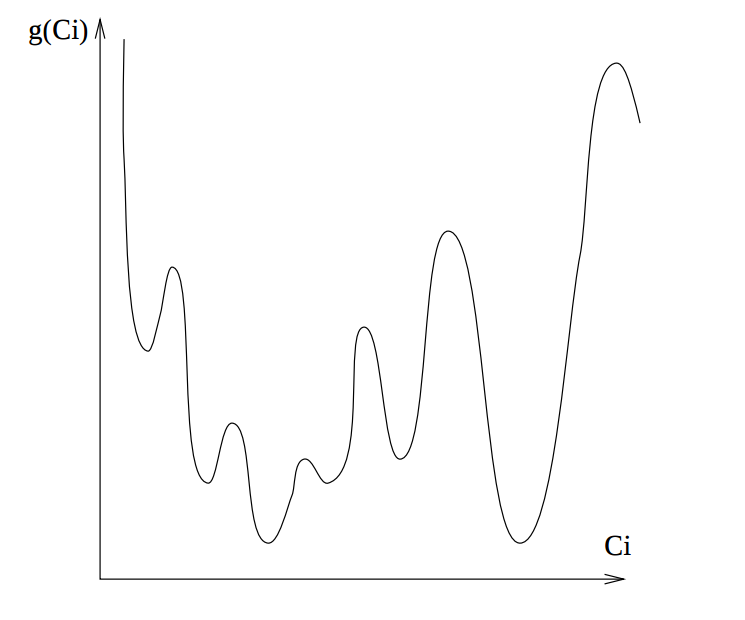
\includegraphics[height=0.9\textheight]{img/18/target_fun}
		\end{figure}
	\end{frame}	
	
%%%%%%%%%%%%%%%%

	\begin{frame}{Typowa funkcja celu}
		Niezbędne:
		\begin{itemize}
			\item $C_i$ - reprezentacja konfiguracji układu
			\item $g(C_i)$
			\item procedura generacji kolejnych konfiguracji
		\end{itemize}
	\end{frame}	
	
%%%%%%%%%%%%%%%%	
	
	\begin{frame}{Przykład procedury generacji nowych konfiguracji}
		\begin{exampleblock}{TSP \cite{lin}}
			Heurystyka: \textit{iterative improvement} - akceptowalne zmiany zmniejszające funkcję celu
			\begin{enumerate}
				\item odwrócenie kolejności obiegu 5-ciu górnych
				\item wstawienie 5-ciu górnych między 2 dolne
			\end{enumerate}	
			$\rightarrow$ pewne ugrzęźnięcie w lokalnym minimum			
			\begin{figure}
				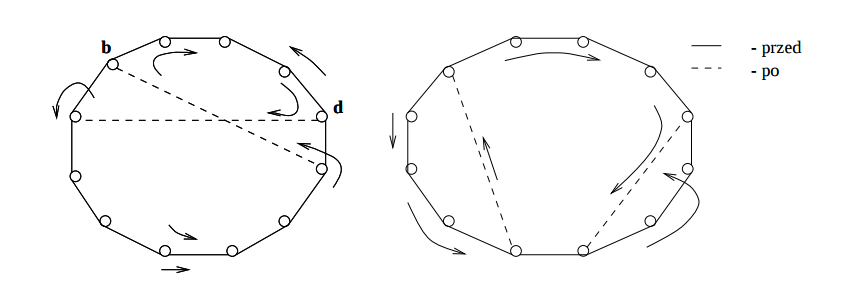
\includegraphics[height=0.4\textheight]{img/18/tsp}
			\end{figure}
		\end{exampleblock}
	\end{frame}
	%%%%%%%%%%%%%%%%%%%%%%%
	\section{Annealing & quenching}

czyli powolne i szybkie schładzanie

Annealing:
- topnienie (ciecz)
- stopniowe, powolne obniżanie temperatury
- w każdej temperaturze długo, do uzyskania równowagi termicznej
=> uporządkowanie w kryształ - struktura regularna, symetryczna o minimalnej energii

Quenching:
- szybkie zmniejszanie temperatury
=> uzyskanie stanu metastabilnego
- szkło
- polikryształ
- kryształ z defektami

odpowiednik iterative improvement

Wniosek: zamiast zawsze odrzucać konfigurację zwiększającą funkcję celu, niekiedy należy ją akceptować z odpowiednim prawdopodobieństwem (uphill)
	%%%%%%%%%%%%%%%%%%%%%%%
	\section{Analogia: fizyka statystyczna - optymalizacja}

Fizyka statystyczna - uśrednione wartości dla zespołów o dużej ilości molekuł

Mechanika statystyczna
- wiele oddziałujących molekuł
- układ, zbiór położeń molekuł 
- schłodzenie do stabilnego stanu niskoenergetycznego
- temperatura
- hamiltonian (energia wewnętrzna)
- w hamiltonianie człony: short-range attractive, long-range repulsive (spin glass)

Optymalizacja
- wiele parametrów
- konfiguracja
- znalezienie konfiguracji prawie optymalnej
- funkcja celu
- współzawodniczące człony funkcji celu

	%%%%%%%%%%%%%%%%%%%%%%%
	\section{Algorytm simulated annealing}

<obrazek>

Ti - temperature schedule: Ti > Ti+1, np. Ti+1 = 0.9 * Ti

Sprawdzanie czy układ jest w równowadze

A)
Utrzymywać Ti przez 
100*N prób
10*N prób udanych (delta g <0)

B)
n - ustalona liczba prób (epoka)
1. wykonać n prób (Ci -> Ci+1)
2. zachować g(Cn)
3. porównać gi(Cn) dla kilku ostatnich zestawów po n próbach -> brak istotej zmiany g(Cn) -> nowe T

Start:
stopienie ->określić typowe delta g, wybrać delta T >> delta g, (delta E)

- Znakomita strona - interaktywna demonstracja działania SA, źródła w C, C++
I DZIAŁA :O
https://www.taygeta.com/annealing/simanneal.html

Programy w C:
Postscript:
% martwe linki
	%%%%%%%%%%%%%%%%%%%%%%%
	\section{Schemat Metropolisa}

%%%%%%%%%%%%%%%%
	\begin{frame}{Schemat Metropolisa}
		\textbf{Podstawa metody Monte Carlo symulacji molekularnej}
		\begin{figure}
			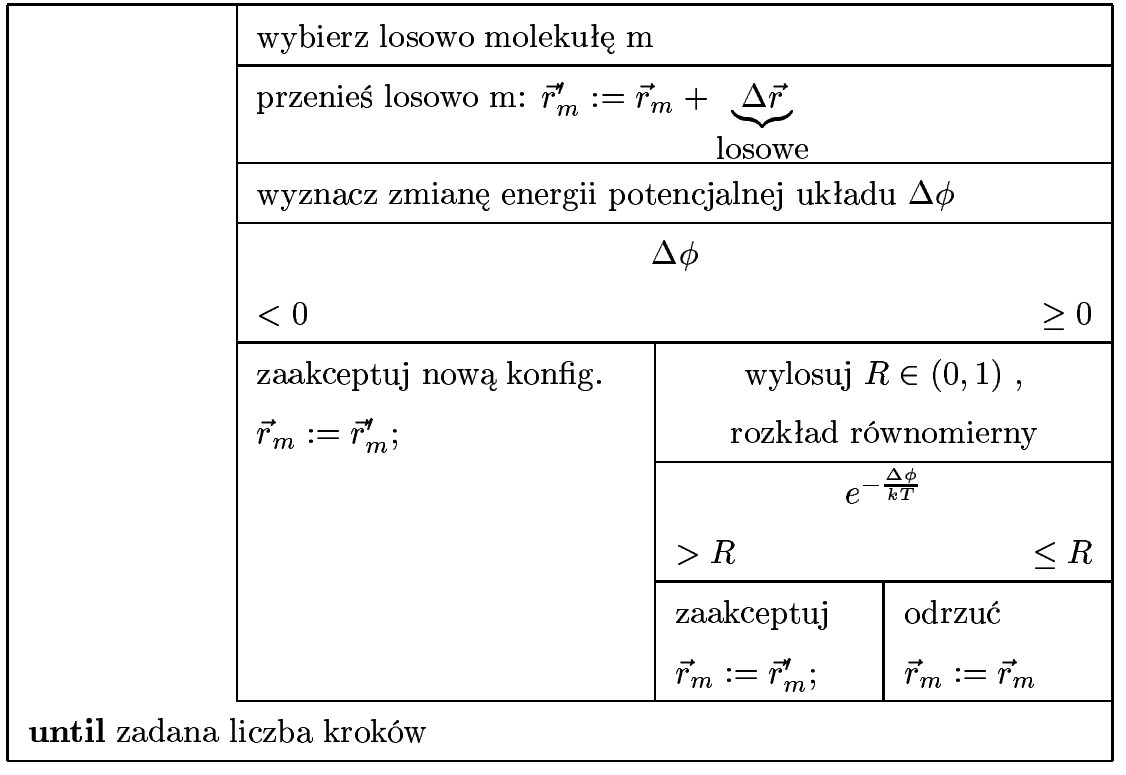
\includegraphics[width=0.67\textwidth]{img/18/metropolis1}
		\end{figure}
		\begin{thebibliography}{9}
			\setbeamertemplate{bibliography item}[article]
			\bibitem{metropolis}{Nicolas Metropolis, Arianna W. Rosenbluth, Marshal M. Rosenbluth, Augusta H. Teller, Edward Teller \newblock J. Chem. Phys. 21 (1953) 1087}
		\end{thebibliography}
	\end{frame}

%%%%%%%%%%%%%%%%

	\begin{frame}{Schemat Metropolisa}
		$$
			\Delta \vec{r} = \delta(\vec{i} \cdot a_x + \vec{j} \cdot a_y  + \vec{k} \cdot a_z)
		$$		
		
		$$
		\delta \text{ - wybrane z góry} \approx 10^{-11}m
		$$		
		
		$$
		a_i \in (-1, 1), Unif
		$$
		
		\begin{figure}
			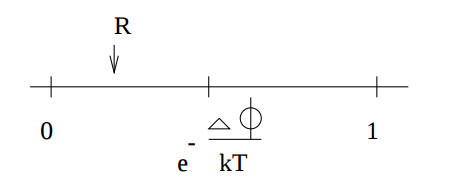
\includegraphics[width=0.5\textwidth]{img/18/metropolis2}
		\end{figure}
		$a_i$, R - liczby pseudolosowe
		
		$\Delta\phi$ - zmiana energii potencjalnej układu w wyniku przesunięcia molekuły m
		
		%Dead link
		%Aplet metropolis/metropolis.html 
	\end{frame}

%%%%%%%%%%%%%%%%
	
	\begin{frame}{Charakterystyka schematu Metropolisa}
		\begin{itemize}
			\item $T \nearrow$ - łatwiej akceptowalne kroki z $H \nearrow (E)$ \\ $ \Rightarrow$ możliwość opuszczenia stanu metastabilnego (lokalnego minimum).
			\item zmiany $H \searrow$ są akceptowane zawsze
		\end{itemize}
		
		Po wielu krokach system $\rightarrow$ stan równowagi termodynamicznej z parametrami oscylującymi wokół wartości średnich zgodnie z rozkładem Boltzmanna
	\end{frame}

\subsection{Łańcuch Markowa}
%%%%%%%%%%%%%%%%
	
	\begin{frame}{Schemat Metropolisa $\rightarrow$ łańcuch Markowa}
		\begin{figure}
				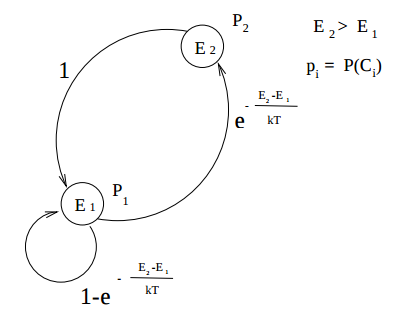
\includegraphics[width=0.5\textwidth]{img/18/markow}
		\end{figure}
		\begin{block}{Zasada równowagi szczegółówej\\ 
		(detailed balance, microscopic reversibility)}
			$$
			p_2 \cdot 1 = p_1 \cdot e^{- \dfrac{E_2 - E_1}{kT}}
			$$
		\end{block}
	\end{frame}

%%%%%%%%%%%%%%%%
	\begin{frame}{Łańcuch Markowa}
		$$
	 	\frac{p1}{p2} = \dfrac{e^{-\frac{E_1}{kT}}}{e^{-\frac{E_2}{kT}}} \rightarrow p_i \sim \underbrace{e^{-\frac{E_i}{kT}}}_{\text{czynnik prawdop. Boltzmanna}}
		$$		
		
		$$
		P(c_i) \sim e^{-\frac{E_i}{kT}}
		$$
		
		$\Rightarrow$ importance sampling: konfiguracje generowane nie losowo - ale z zadanym rozkładem (50-70 \% akceptowanych)
		%Dead link
		%	Notatka nt. niejednorodnych łańcuchów Markowa w SA, dużo bibliografii
		
		% whaaaat
		% http://www.pz.zgora.pl/discuss/al15_2/a6.htm
		
	\end{frame}
	
\section{Uwagi praktyczne}
%%%%%%%%%%%%%%%%
	\begin{frame}{Uwagi praktyczne}
		\textbf{Duże $\Delta\vec{r}$:}
		\begin{itemize}
			\item niski poziom akceptacji
			\item szybsze próbkowanie przestrzeni konfiguracyjnej
		\end{itemize}
		
		\textbf{Dla potencjałów parowych, krótkozasięgowych:}
		\begin{itemize}
			\item przesuwamy tylko 1 cząstkę
			\item dla określenia $\Delta\phi$ - tylko najbliżsi sąsiedzi
		\end{itemize}
		
		\textbf{W przypadku cieczy:}
		\begin{itemize}
			\item każda cząsteczka $\approx 10^3$ przemieszczeń
			\item w modelu $\approx 10^3$ cząsteczek
		\end{itemize}	
		
		\textbf{Force-biased displacement:}
		\begin{itemize}
			\item wszystkie cząsteczki przesuwane równocześnie przeciwnie do gradientu potencjału
		\end{itemize}
		
	\end{frame}

	%%%%%%%%%%%%%%%%%%%%%%%
	\section{Simulated Annealing a rozkład kanoniczny}

- własności makroskopowe z mikroskopowymi
Q - stan mikroskopowy układu
E(Q) - energia ukłądu w stanie Q
P(Q) - rozkład prawdopodobieństwa 
Rozkład mikrokanoniczny - układ izolowany

$$
P(Q) = A(Q) \cdot \delta(E - E(Q))
A(Q) = \begin{cases}
0 - \text{niemożliwe} \\
A - \text{możliwe}
\end{cases}
$$

Rokład kanoniczny - ukłąd w kontakcie cieplnym z otoczeniem
<obrazek>

$$
P(Q) = Z^{-1} \cdot e^{-\frac{E(Q)}{kT}}
$$

$$
\sum_Q P(Q) = Z^{-1} \cdot \sum_Q ^{-\frac{E(Q)}{kT}} = 1 \rightarrow Z = \underarrow{suma statystyczna - funkcja rozdziału $\rightarrow$ bardzo ważna!}{\sum_Q ^{-\frac{E(Q)}{kT}}}
$$

często: $\frac{1}{kT} = \beta$

E = Var
<E> = U $\rightarrow$ energia wewnętrzna: można ją zmierzyć

$$
<E> = \sum_Q E(Q) \cdot P(Q) = \dfrac{\sum_Q E(Q) \cdot e^{-\beta\cdot E(Q)}}{\sum_Q e^{-\beta\cdotE(Q)}} = - \frac{\partial}{\partial \beta} ln Z
$$

$$
<E> = \frac{\partial}{\partial \beta} ln Z
$$

Ciepło właściwe przy stałej objętości:

$$
C_v = \frac{d<E(T)>}{dT}
$$

ale:

$$
c_v = \frac{k}{\beta^2}[\underbraces{średni kwadrat energii}{<E^2(T)>} - \underbraces{kwadrat średniej energii	}{<E(T)>^2}] 
$$

Wzrost wartości ciepła właściwego sygnalizuje zachodzenie przemiany fazowej.
S - entropia układu:

$$
T \cdot dS = dQ - ciepło dostarczane układowi
$$

$$
V = const
$$

$$
T \cdot dS = dU = C_v \cdot dT \rightarrow \frac{ds}{dT} = \frac{C_v(T)}{T}
$$

$$
S(T) = S(T_1) - \int_T^{T_1} \frac{C_v(T')}{T'}dT'
$$

$T_1$ - temperatura, dla której entropia jest znana (np. przez aproksymację dla b. wysokich temperatur)
Poziom S $\rightarrow$ ilość minimów (stanów ustalonych)


	%%%%%%%%%%%%%%%%%%%%%%%
	\section{Pierwsze zastosowania Simulated Annealing}

Kirkpatrick

TSP - 3000 random cities (dokładne rozwiązanie $\leq$ 318) - miasta w klastrach:
- duże T - optymalna droga między klastrami
- małe T - optymalna droga wewnątrz klastrów

$\rightarrow$ "divide and conquer" behaviour $\rightarrow$ podział zagadnienia na różne skale

Kirkpatrick, Gelatt

Optymalizacja rozłożenia mikroukładów elektronicznych na 1 lub więcej chipach, łączenie chipów.

Vecchi, Kirkpatrick

$\rightarrow$ optimal wiring (między VLSI)
- min length
- min bends
- no crowding

Kenneth Wilson, Dean Jacobs, Jan Prins - Cornell University

Algorytm Metropolisa do optymalizacji kodu komputerowego ($\approx$ iteracyjne przestawianie komend)

% Dead links:
% Simulated annealing jako przykład metody wyszukiwania
% http://yoda.cis.temple.edu:8080/UGAIWWW/lectures95/search/more-search.html#4

% Zastosowania Simulated Annealing w biologii molekularnej
% http://ams.sunysb.edu/~deng/korobka/index.html
	%%%%%%%%%%%%%%%%%%%%%%%
	\section{Odmiany Simulated Annealing}
	\begin{frame}{Odmiany Simulated Annealing}
		\begin{itemize}
			%Mostly dead
			%COSA - Cooperative Simulated Annealing
			%Program w Javie implementujący COSA:
			%https://www.wiwi.uni-frankfurt.de/~stockhei/newcosa/index.html
			
			\item \textbf{ASA - Adaptive Simulated Annealing}\\			
			Strona prof. Lester Ingbera poświęcona ASA:\\
				\url{http://alumnus.caltech.edu/~ingber/}
			
			%Materiały na temat ASA:
			%ftp.alumni.caltech.edu
			
			%Inny serwer ftp z materiałami dotyczącymi ASA:
			%ftp://almond.srv.cs.cmu.edu/
			
			%PARSA - Parallel Simulated Annealing
			%ftp://almond.srv.cs.cmu.edu/~parsa
			
			%EBSA - Ensemble Based Simulated Annealing
			%http://sdsc.edu/~frost/Ebsa/Ebsa.html
		\end{itemize}

		
	\end{frame}
	%%%%%%%%%%%%%%%%%%%%%%%
	\section{Literatura}

\begin{frame}[allowframebreaks]{Literatura}
	\begin{thebibliography}{9}
		\setbeamertemplate{bibliography item}[article]
            \bibitem{kirkpatrick}{Scott Kirkpatrick, Daniel Gelatt, Mario Venchi \newblock IBM T.J. Watson Research Center \newblock Science 220 (1983) 671-670 }
		\setbeamertemplate{bibliography item}[article]
            \bibitem{kirkpatrick}{S. Kirkpatrick \newblock J. Stat. Phys. 34 (1984) 975 (No 5/6)}
     	\setbeamertemplate{bibliography item}[article]
                 \bibitem{garey}{M.R. Garey, D.S. Johnson \newblock Computers and Intractability: A Guide to the Theory of NP \newblock Completeness, Freeman, San Francisco, 1979}
         \setbeamertemplate{bibliography item}[book]
                          \bibitem{lin}{S. Lin, B.W. Kernighan \newblock Oper. Res. 21 (1973) 498}
         \setbeamertemplate{bibliography item}[article]
                                   \bibitem{metropolis}{Nicolas Metropolis, Arianna W. Rosenbluth, Marshal M. Rosenbluth, Augusta H. Teller, Edward Teller \newblock J. Chem. Phys. 21 (1953) 1087}
    \end{thebibliography}
\end{frame}
\end{document}
